% CS615 Aspects of System Administration
% Author: Jan Schaumann <jschauma@netmeister.org>

\documentclass[xga]{xdvislides}
\usepackage[landscape]{geometry}
\usepackage{graphics}
\usepackage{graphicx}
\usepackage{colordvi}

\newcommand{\smallish}{\fontsize{18}{18}\selectfont}

\begin{document}
\setfontphv

%%% Headers and footers
\lhead{\slidetitle}				% default:\lhead{\slidetitle}
\chead{CS615 - Aspects of System Administration}% default:\chead{\relax}
\rhead{Slide \thepage}				% default:\rhead{\sectiontitle}
\lfoot{\Gray{Lecture 01: Introduction}}		% default:\lfoot{\slideauthor}
\cfoot{\relax}					% default:\cfoot{\relax}
\rfoot{\Gray{\today}}

\vspace*{\fill}
\begin{center}
	\Hugesize
		CS615 - Aspects of System Administration\\ [1em]
	\hspace*{5mm}\blueline\\ [1em]
	\Normalsize
		Department of Computer Science\\
		Stevens Institute of Technology\\
		Jan Schaumann\\
		\verb+jschauma@stevens.edu+ \\
		\verb+http://www.cs.stevens.edu/~jschauma/615/+
\end{center}
\vspace*{\fill}

\subsection{New Rules}
\Hugesize
\vspace*{\fill}
\begin{center}
Close your laptops!
\end{center}
\vspace*{\fill}
\Normalsize

\subsection{New Rules}
\Hugesize
\vspace*{\fill}
\begin{center}
Close your laptops! \\
\vspace{.5in}
Open your eyes! \\
\small
(Mind, too.)
\end{center}
\vspace*{\fill}
\Normalsize



\subsection{The Job of a System Administrator}
What {\bf exactly} does a {\em System Administrator} do?

\subsection{The Job of a System Administrator}
\vspace*{\fill}
\begin{center}
	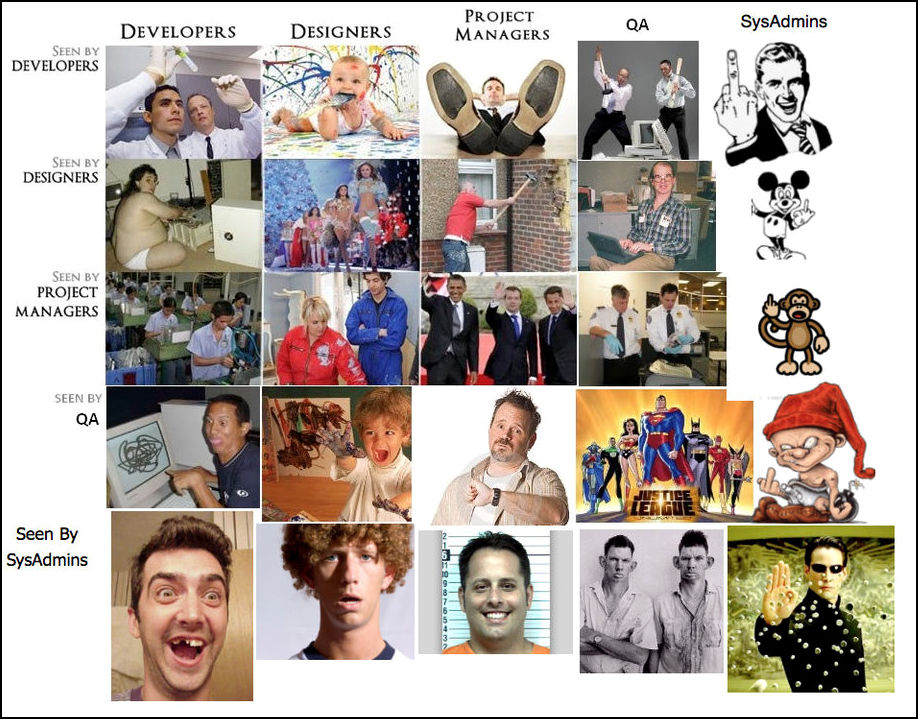
\includegraphics[scale=0.45]{pics/as-seen-by.eps} \\
\end{center}
\vspace*{\fill}

\subsection{The Job of a System Administrator}
\begin{center}
	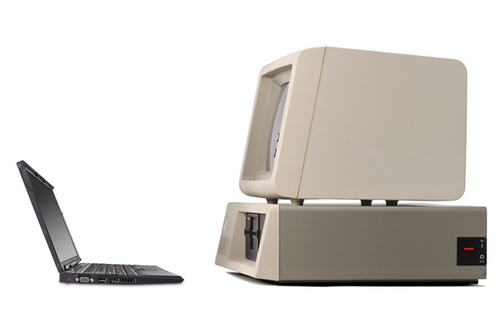
\includegraphics[scale=0.9]{pics/computers.eps} \\
\end{center}

\subsection{The Job of a System Administrator}
\vspace*{\fill}
\begin{center}
	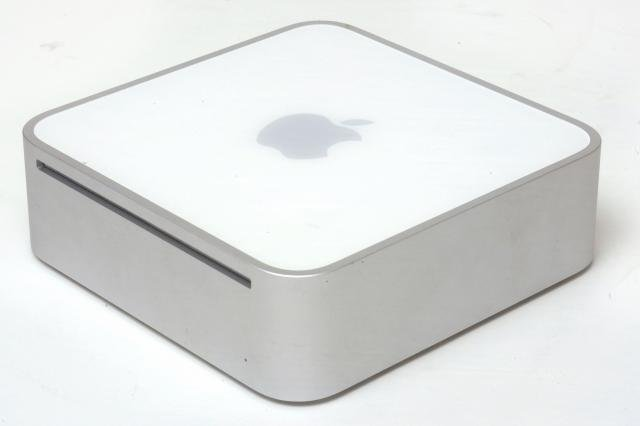
\includegraphics[scale=0.6]{pics/macmini.eps} \\
\end{center}
\vspace*{\fill}

\subsection{The Job of a System Administrator}
\vspace*{\fill}
\begin{center}
	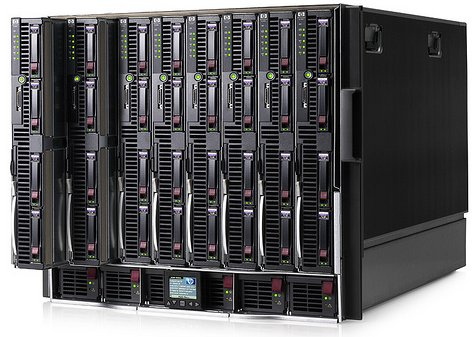
\includegraphics[scale=1.2]{pics/blades.eps} \\
\end{center}
\vspace*{\fill}

\subsection{The Job of a System Administrator}
\vspace*{\fill}
\begin{center}
	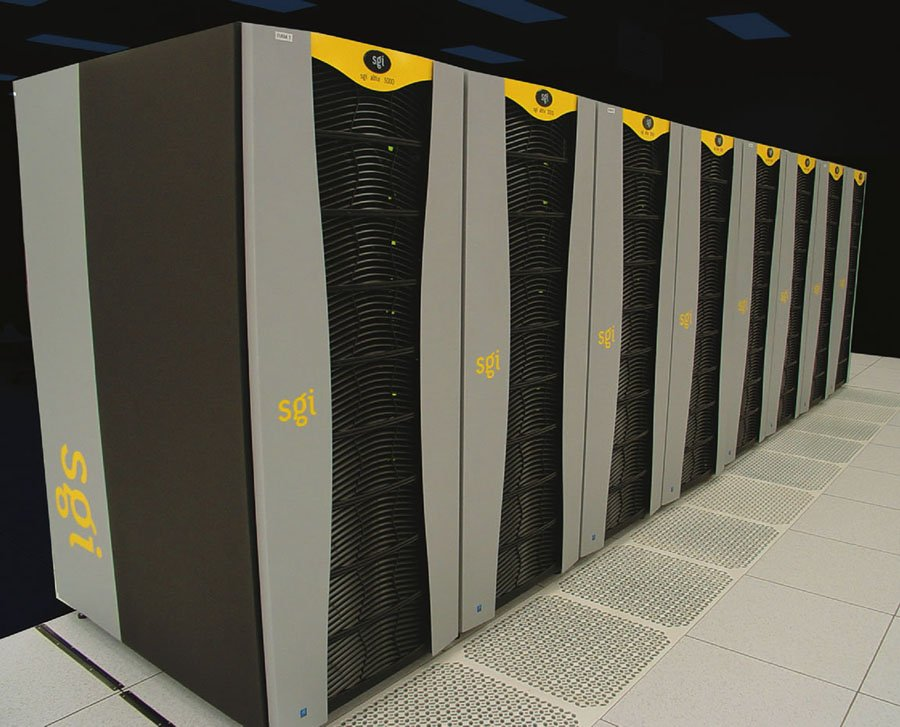
\includegraphics[scale=0.4]{pics/altix.eps} \\
\end{center}
\vspace*{\fill}

\subsection{The Job of a System Administrator}
\vspace*{\fill}
\begin{center}
	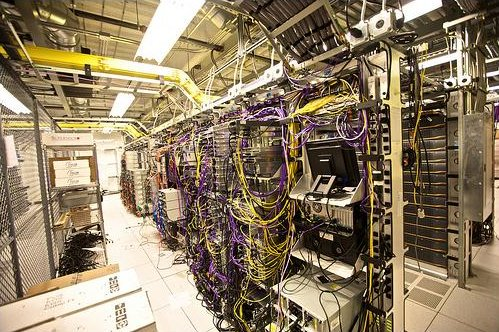
\includegraphics[scale=0.9]{pics/datacenter.eps} \\
\end{center}
\vspace*{\fill}

\subsection{The Job of a System Administrator}
\vspace*{\fill}
\begin{center}
	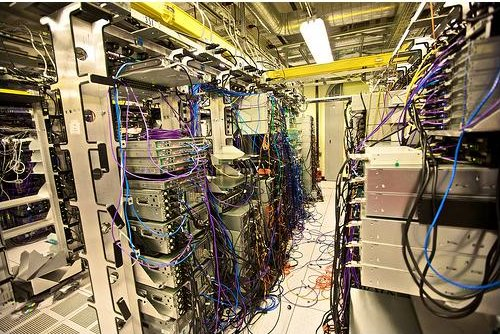
\includegraphics[scale=0.9]{pics/datacenter2.eps} \\
\end{center}
\vspace*{\fill}

\subsection{The Job of a System Administrator}
\vspace*{\fill}
\begin{center}
	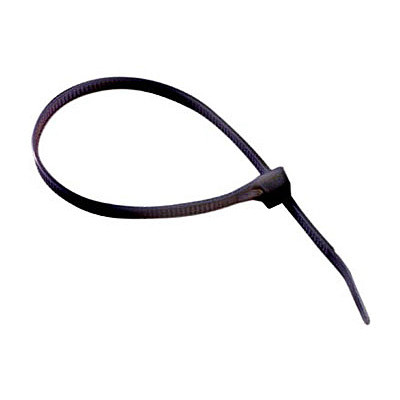
\includegraphics[scale=0.7]{pics/Cable_Tie.eps} \\
\end{center}
\vspace*{\fill}

\subsection{The Job of a System Administrator}
\vspace*{\fill}
\begin{center}
	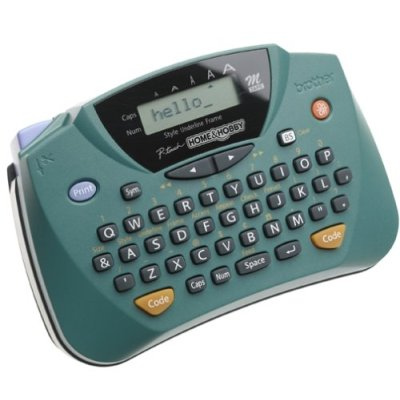
\includegraphics[scale=0.7]{pics/labelmaker.eps} \\
\end{center}
\vspace*{\fill}

\subsection{The Job of a System Administrator}
\vspace*{\fill}
\begin{center}
	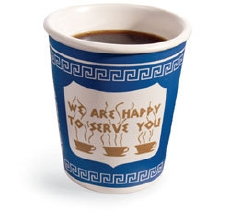
\includegraphics[scale=1.2]{pics/coffee.eps} \\
\end{center}
\vspace*{\fill}

\subsection{The Job of a System Administrator}
\vspace*{\fill}
\begin{center}
	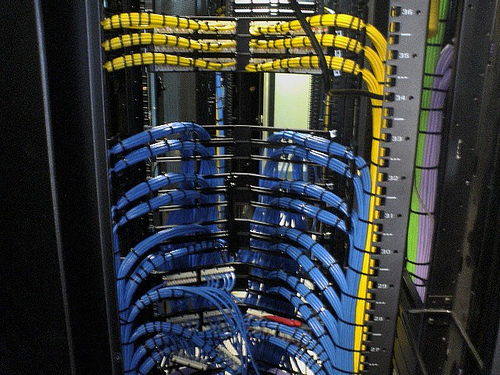
\includegraphics[scale=0.8]{pics/cables2.eps} \\
\end{center}
\vspace*{\fill}

\subsection{The Job of a System Administrator}
\vspace*{\fill}
\begin{center}
	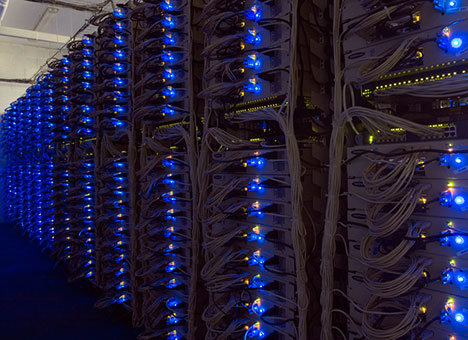
\includegraphics[scale=1.2]{pics/data-center-servers-t001.eps} \\
\end{center}
\vspace*{\fill}

\subsection{The Job of a System Administrator}
\vspace*{\fill}
\begin{center}
	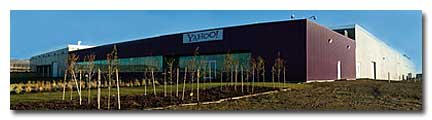
\includegraphics[scale=2.0]{pics/quincy-panorama.eps} \\
\end{center}
\vspace*{\fill}

\subsection{The Job of a System Administrator}
\vspace*{\fill}
\begin{center}
	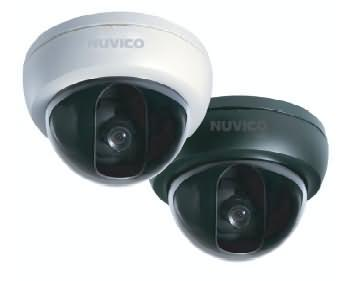
\includegraphics[scale=0.9]{pics/camera.eps} \\
\end{center}
\vspace*{\fill}

\subsection{The Job of a System Administrator}
\vspace*{\fill}
\begin{center}
	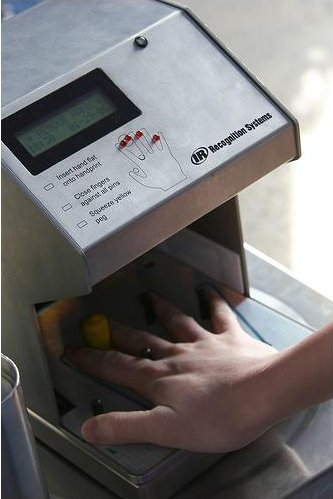
\includegraphics[scale=0.6]{pics/hand-scanner.eps} \\
\end{center}
\vspace*{\fill}

\subsection{The Job of a System Administrator}
\vspace*{\fill}
\begin{center}
	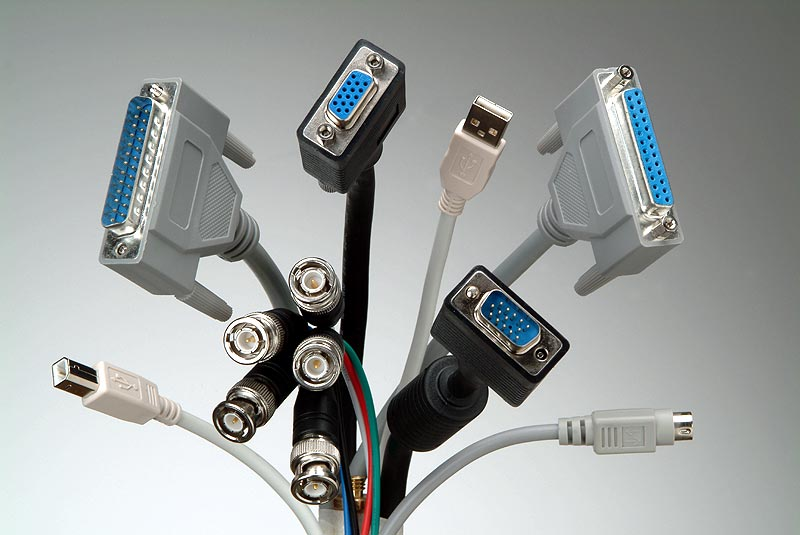
\includegraphics[scale=0.7]{pics/computer-cables-big.eps} \\
\end{center}
\vspace*{\fill}

\subsection{The Job of a System Administrator}
\vspace*{\fill}
\begin{center}
	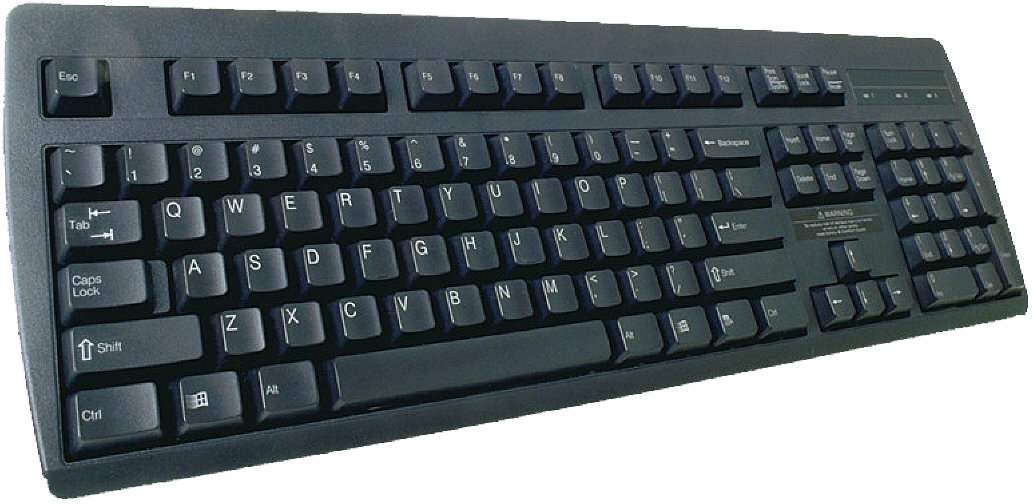
\includegraphics[scale=4.0]{pics/keyboard.eps} \\
\end{center}
\vspace*{\fill}

\subsection{The Job of a System Administrator}
\vspace*{\fill}
\begin{center}
	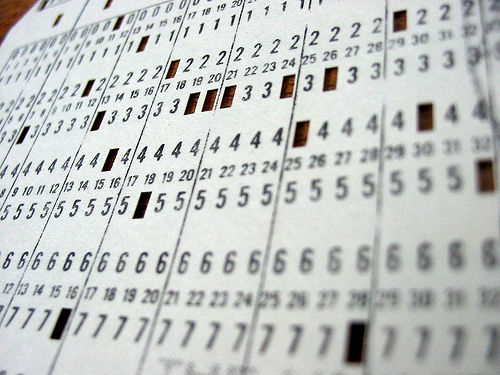
\includegraphics[scale=0.7]{pics/punchcard.eps} \\
\end{center}
\vspace*{\fill}

\subsection{The Job of a System Administrator}
\vspace*{\fill}
\begin{center}
	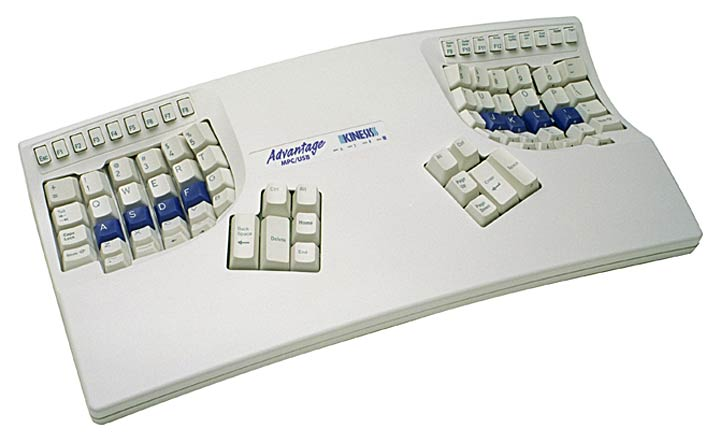
\includegraphics[scale=0.9]{pics/kinesis.eps} \\
\end{center}
\vspace*{\fill}

\subsection{The Job of a System Administrator}
\vspace*{\fill}
\begin{center}
	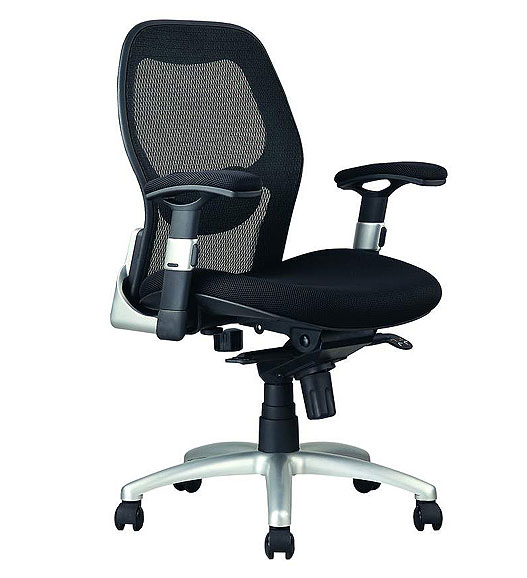
\includegraphics[scale=0.65]{pics/office-chair.eps} \\
\end{center}
\vspace*{\fill}

\subsection{The Job of a System Administrator}
\vspace*{\fill}
\begin{center}
	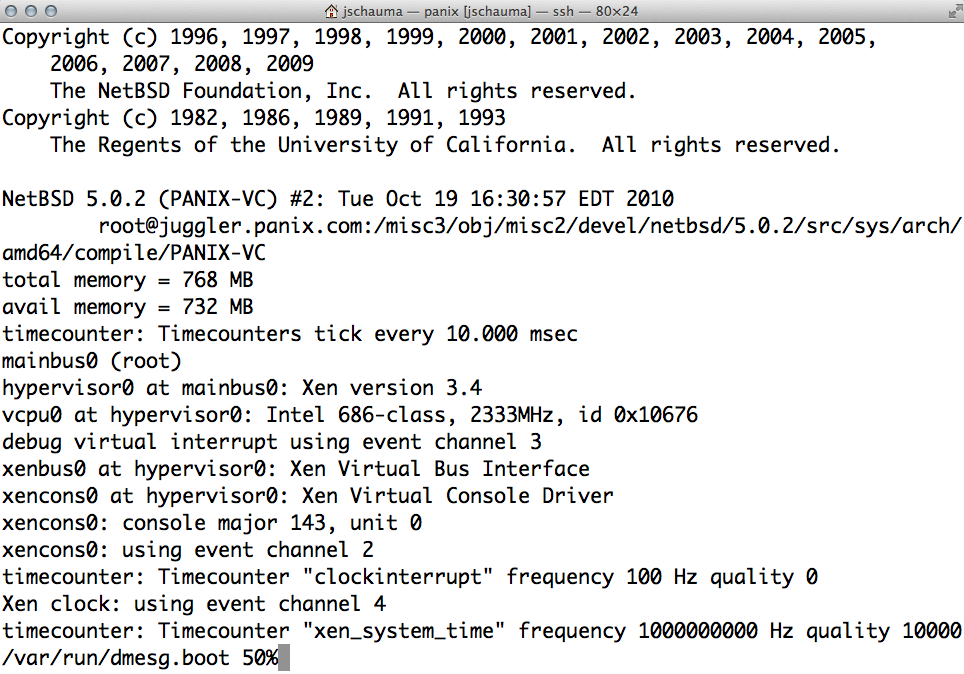
\includegraphics[scale=0.4]{pics/dmesg.eps} \\
\end{center}
\vspace*{\fill}

\subsection{The Job of a System Administrator}
\vspace*{\fill}
\begin{center}
	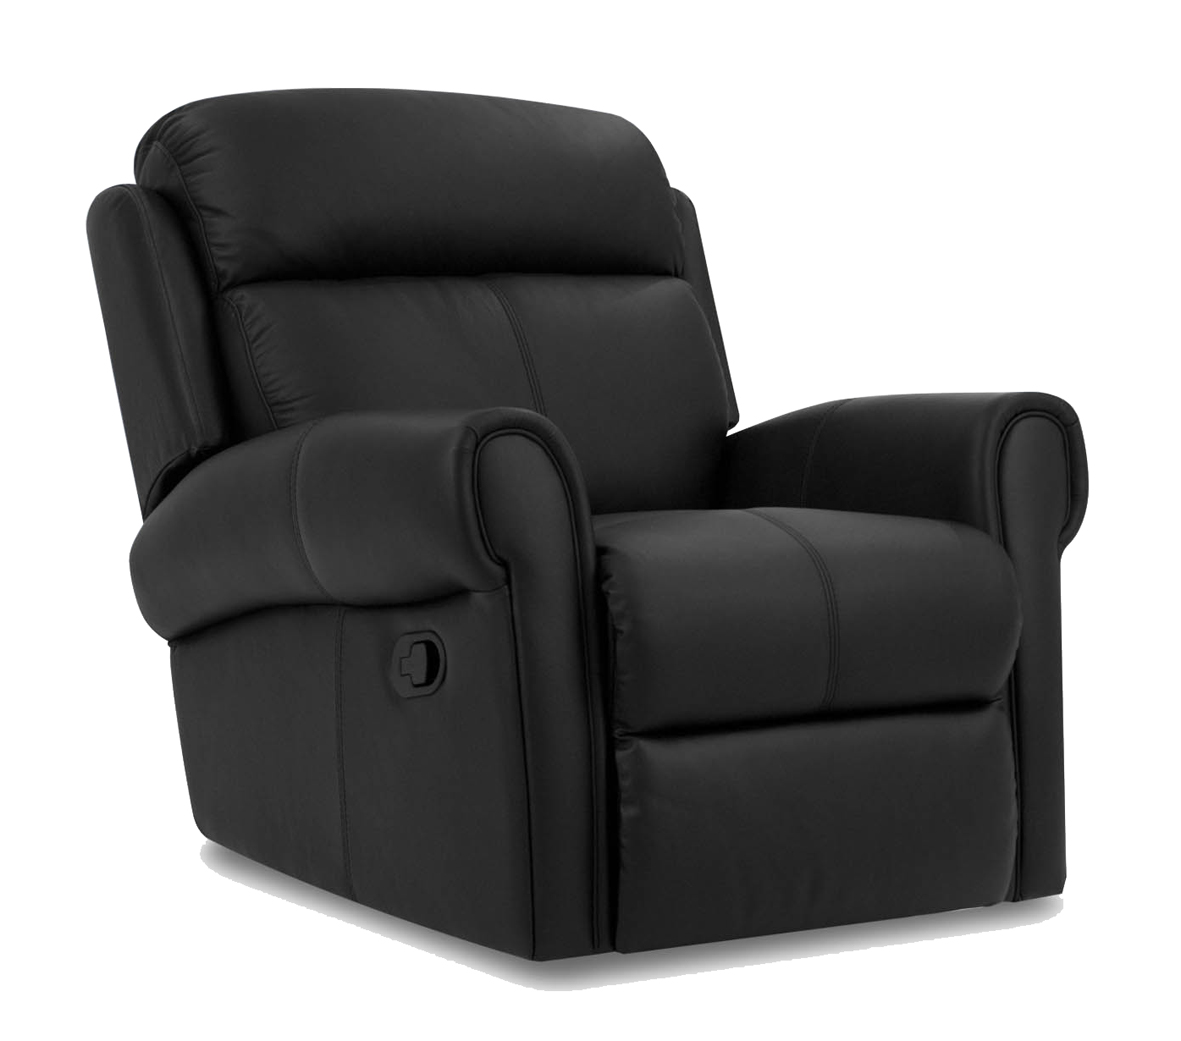
\includegraphics[scale=1.1]{pics/armchair.eps} \\
\end{center}
\vspace*{\fill}

\subsection{The Job of a System Administrator}
\vspace*{\fill}
\begin{center}
	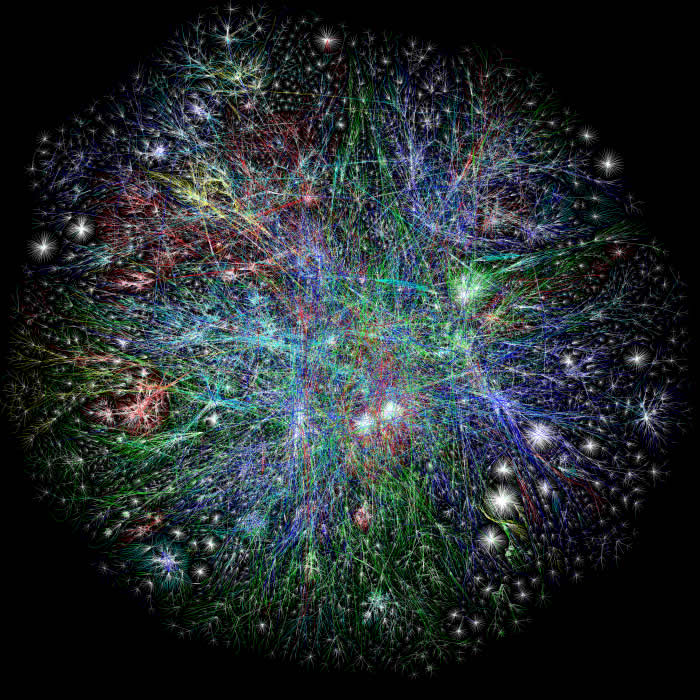
\includegraphics[scale=0.4]{pics/internet.eps} \\
	\small
	{\tt http://www.opte.org/maps/}
	\Normalsize
\end{center}
\vspace*{\fill}

\subsection{The Job of a System Administrator}
\vspace*{\fill}
\begin{center}
	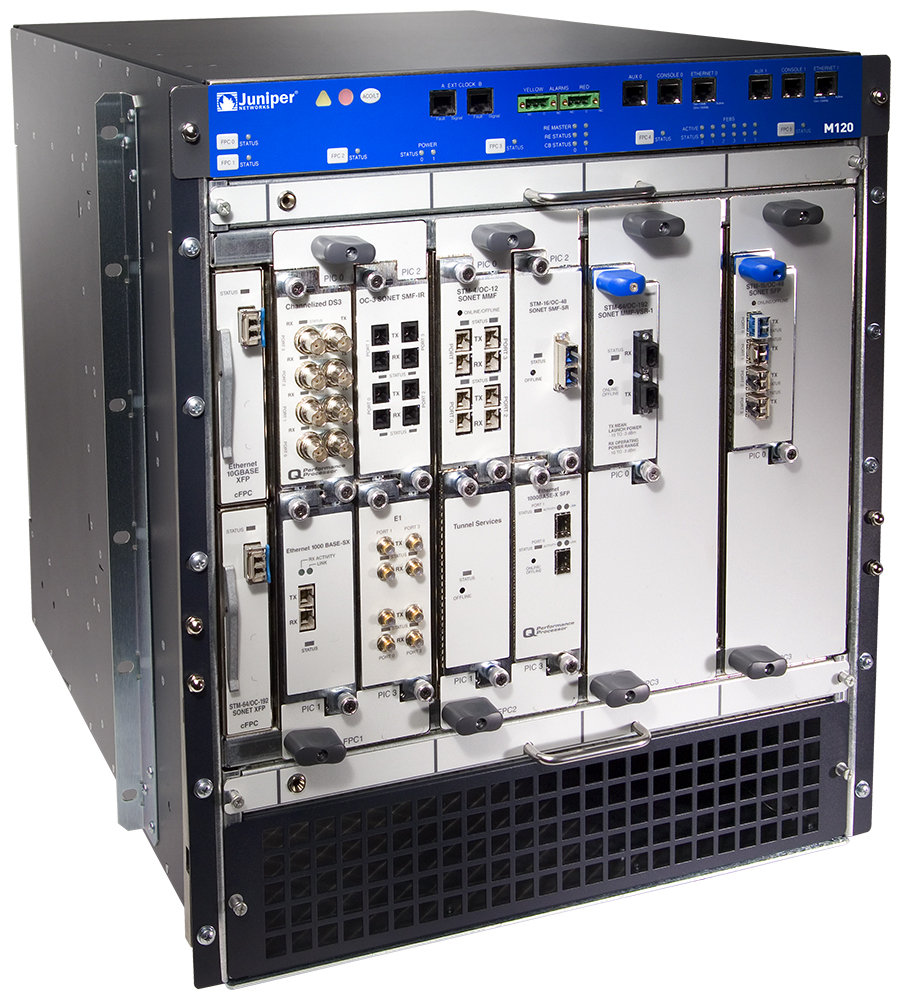
\includegraphics[scale=0.35]{pics/juniper.eps} \\
\end{center}
\vspace*{\fill}

\subsection{The Job of a System Administrator}
\vspace*{\fill}
\begin{center}
	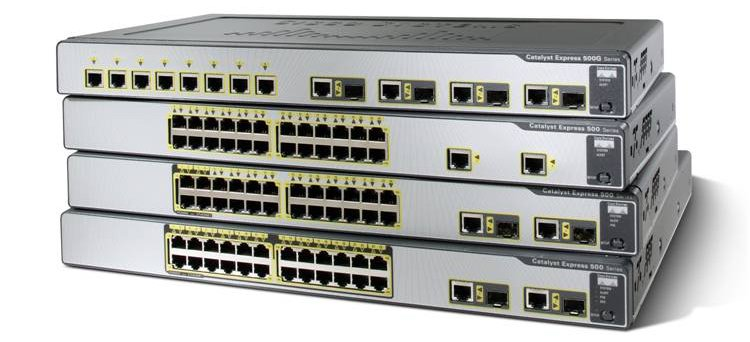
\includegraphics[scale=1.6]{pics/switches.eps} \\
\end{center}
\vspace*{\fill}

\subsection{The Job of a System Administrator}
\vspace*{\fill}
\begin{center}
	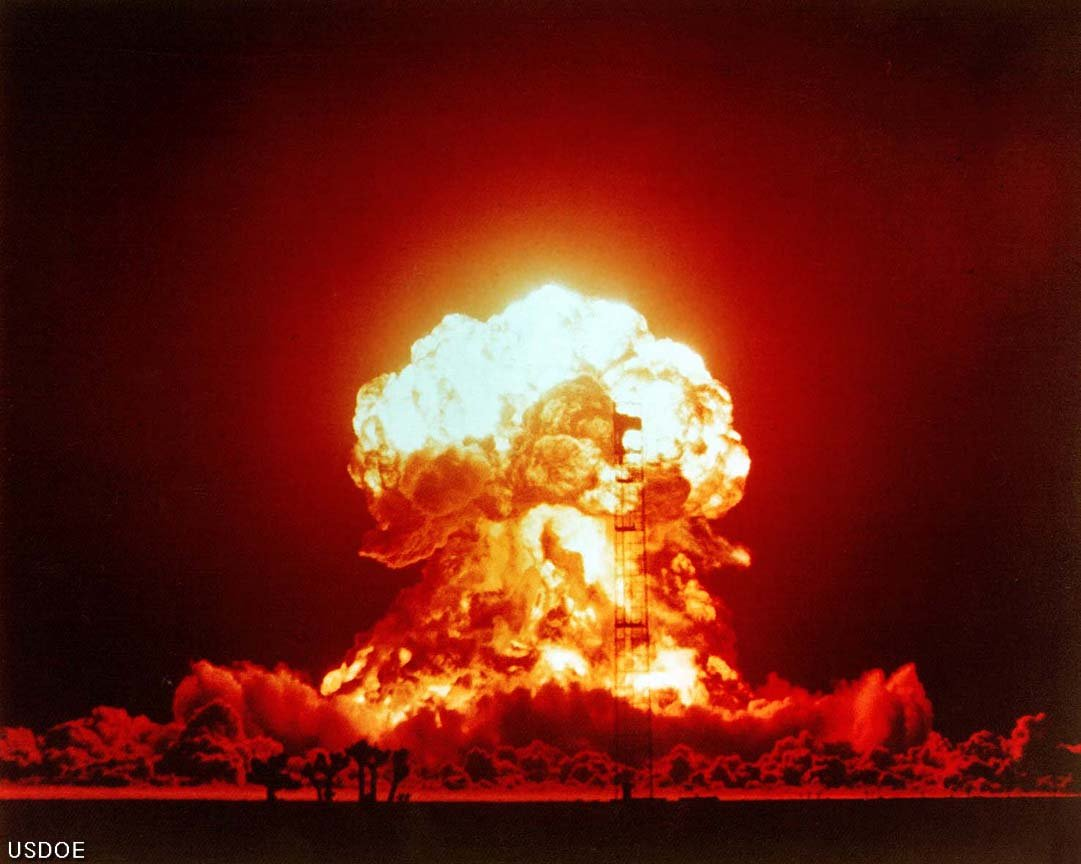
\includegraphics[scale=0.4]{pics/mushroom_cloud.eps} \\
\end{center}
\vspace*{\fill}

\subsection{The Job of a System Administrator}
\vspace*{\fill}
\begin{center}
	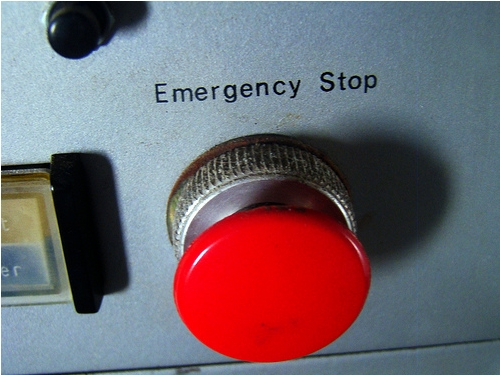
\includegraphics[scale=0.8]{pics/big-red-button.eps} \\
\end{center}
\vspace*{\fill}

\subsection{The Job of a System Administrator}
\vspace*{\fill}
\begin{center}
	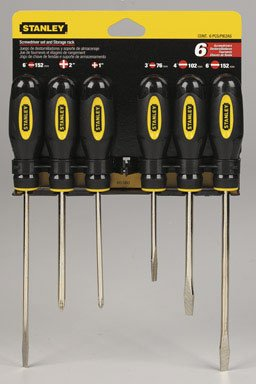
\includegraphics[scale=0.75]{pics/screwdrivers.eps} \\
\end{center}
\vspace*{\fill}

\subsection{The Job of a System Administrator}
\vspace*{\fill}
\begin{center}
	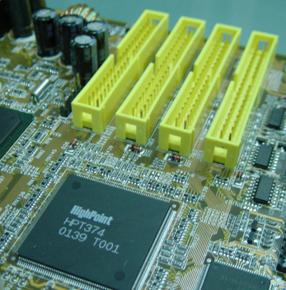
\includegraphics[scale=1.2]{pics/raid.eps} \\
\end{center}
\vspace*{\fill}

\subsection{The Job of a System Administrator}
\vspace*{\fill}
\begin{center}
	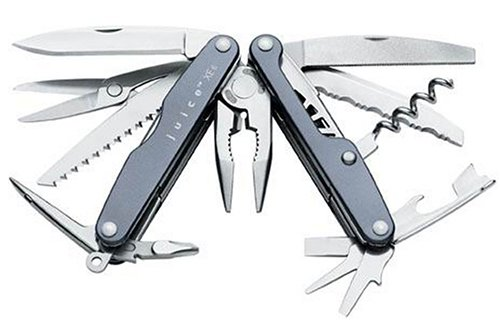
\includegraphics[scale=0.85]{pics/leatherman.eps} \\
\end{center}
\vspace*{\fill}

\subsection{The Job of a System Administrator}
\vspace*{\fill}
\begin{center}
	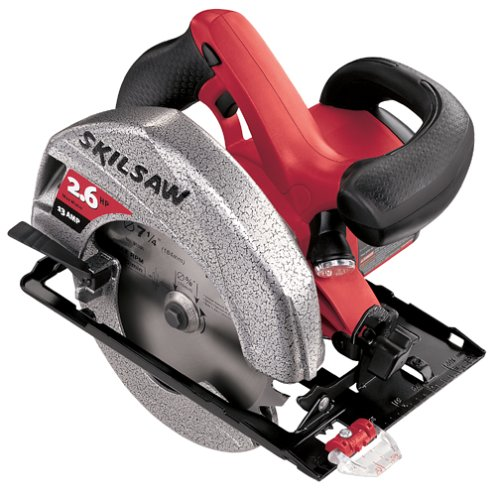
\includegraphics[scale=0.5]{pics/circularsaw.eps} \\
	\small See also: {\tt http://is.gd/WUezLL} \Normalsize
\end{center}
\vspace*{\fill}

\subsection{The Job of a System Administrator}
\vspace*{\fill}
\begin{center}
	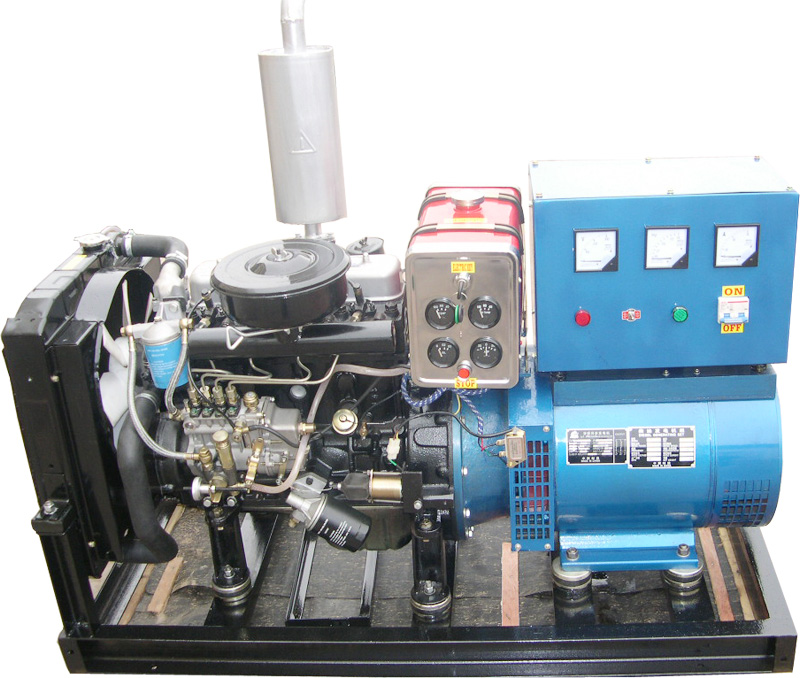
\includegraphics[scale=1.9]{pics/diesel-generator.eps} \\
\end{center}
\vspace*{\fill}

\subsection{The Job of a System Administrator}
\vspace*{\fill}
\begin{center}
	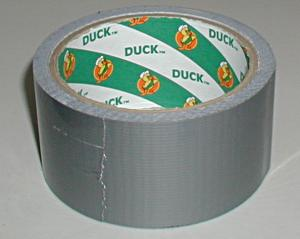
\includegraphics[scale=1.1]{pics/DuckTape.eps} \\
\end{center}
\vspace*{\fill}
\subsection{The Job of a System Administrator}
\vspace*{\fill}
\begin{center}
	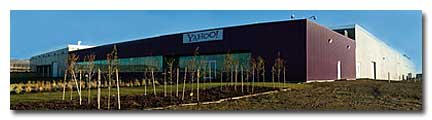
\includegraphics[scale=2.0]{pics/quincy-panorama.eps} \\
\end{center}
\vspace*{\fill}

\subsection{The Job of a System Administrator}
\vspace*{\fill}
\begin{center}
	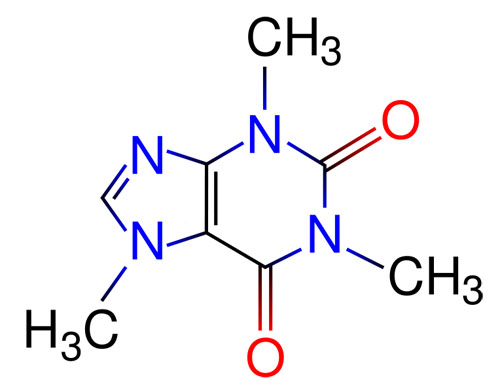
\includegraphics[scale=0.65]{pics/Caffeine_molecule.eps} \\
\end{center}
\vspace*{\fill}

\subsection{The Job of a System Administrator}
\vspace*{\fill}
\begin{center}
	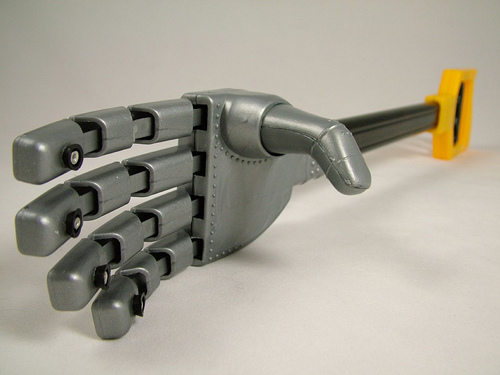
\includegraphics[scale=0.7]{pics/remote_hands.eps} \\
\end{center}
\vspace*{\fill}

\subsection{The Job of a System Administrator}
\vspace*{\fill}
\begin{center}
	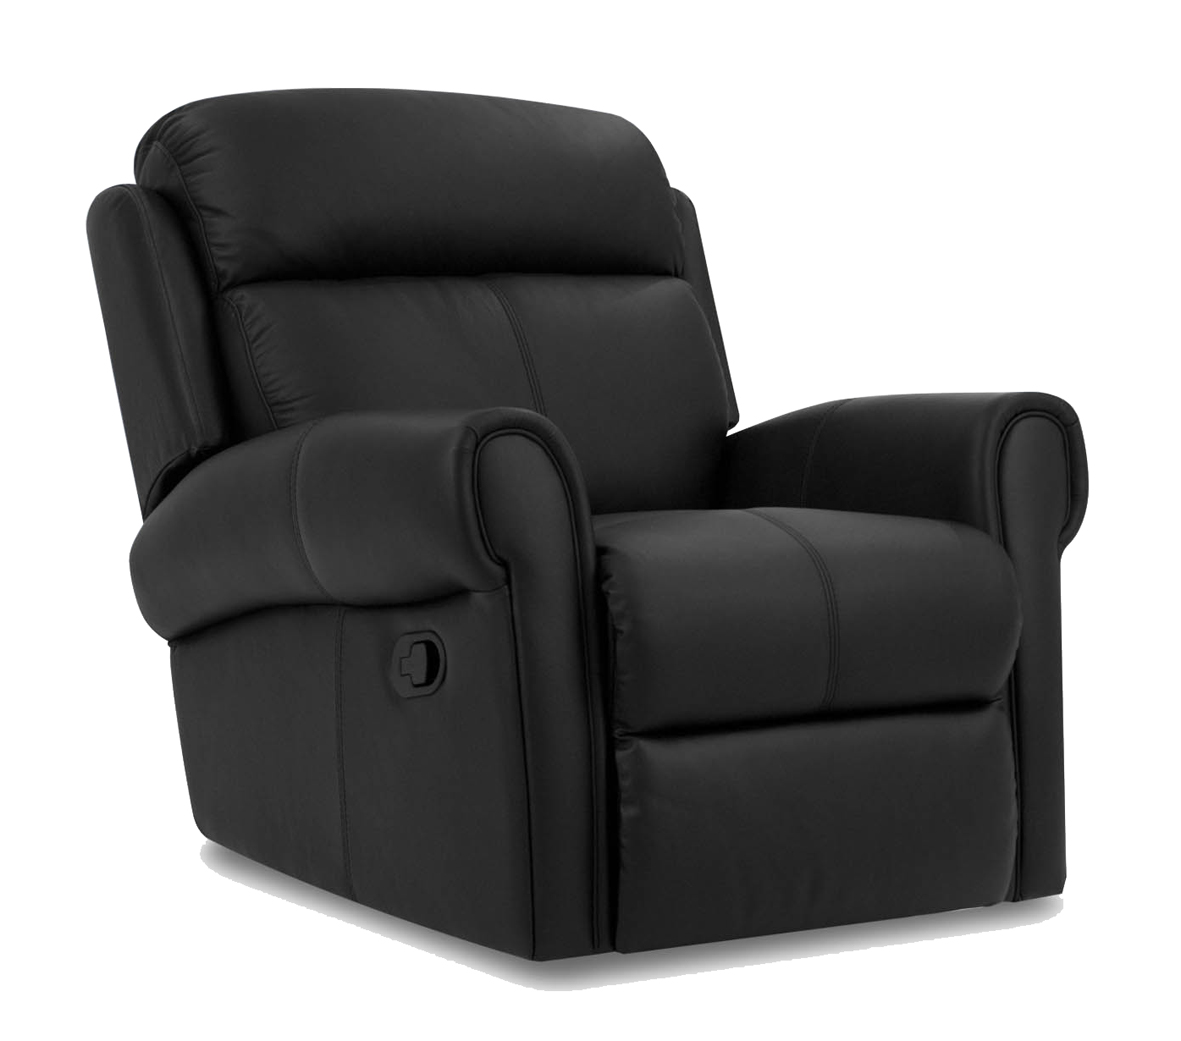
\includegraphics[scale=1.1]{pics/armchair.eps} \\
\end{center}
\vspace*{\fill}

\subsection{The Job of a System Administrator}
\vspace*{\fill}
\begin{center}
	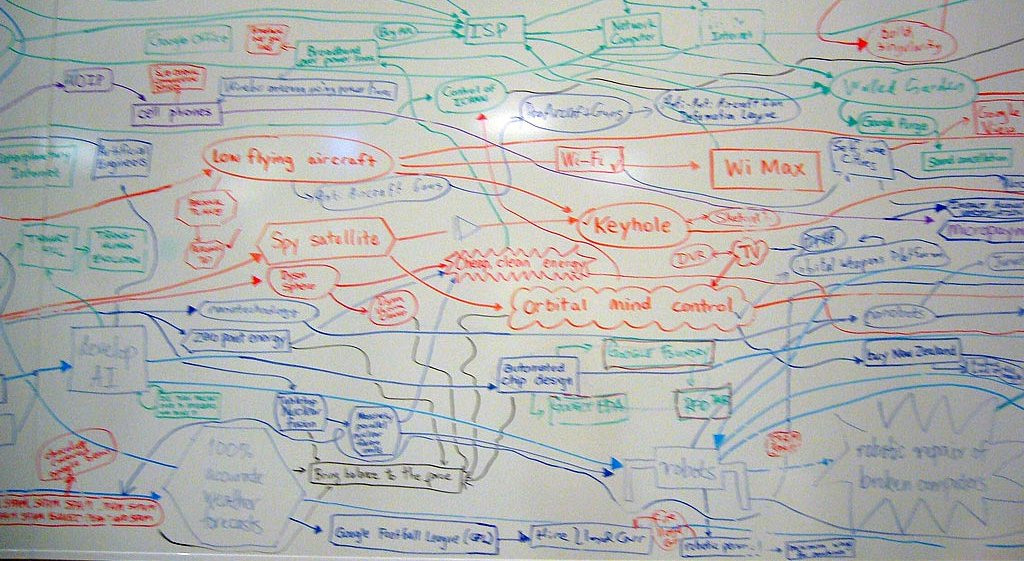
\includegraphics[scale=0.52]{pics/google_whiteboard_large.eps} \\
\end{center}
\vspace*{\fill}

\subsection{The Job of a System Administrator}
\vspace*{\fill}
\begin{center}
	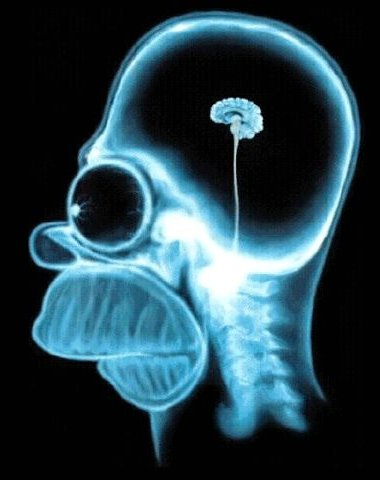
\includegraphics[scale=0.7]{pics/homer-brain.eps} \\
\end{center}
\vspace*{\fill}

\subsection{The Job of a System Administrator}
What {\bf exactly} does a {\em System Administrator} do?

\subsection{The Job of a System Administrator}
What {\bf exactly} does a {\em System Administrator} do?
\begin{itemize}
	\item no precise job description
\end{itemize}

\subsection{The Job of a System Administrator}
What {\bf exactly} does a {\em System Administrator} do?
\begin{itemize}
	\item no precise job description
\end{itemize}

	\begin{center}
		
\includegraphics[scale=1.0]{pics/matrix.eps} \\
	\end{center}




\subsection{The Job of a System Administrator}
What {\bf exactly} does a {\em System Administrator} do?
\begin{itemize}
	\item no precise job description
\end{itemize}
\vfill
 system administrator n.: \\
{\em one who, as a primary job function,
	manages computer and network systems on behalf of another, such as an
	employer or client.}

\subsection{The Job of a System Administrator}
What {\bf exactly} does a {\em System Administrator} do?
\begin{itemize}
	\item no precise job description
	\item often learned by experience
\end{itemize}
\vfill
system administrator n.: \\
{\em one who, as a primary job function,
	manages computer and network systems on behalf of another, such as an
	employer or client.}

\subsection{The Job of a System Administrator}
What {\bf exactly} does a {\em System Administrator} do?
\begin{itemize}
	\item no precise job description
	\item often learned by experience
	\item ``makes things run''
\end{itemize}
\vfill
system administrator n.: \\
{\em one who, as a primary job function,
	manages computer and network systems on behalf of another, such as an
	employer or client.}

\subsection{The Job of a System Administrator}
What {\bf exactly} does a {\em System Administrator} do?
\begin{itemize}
	\item no precise job description
	\item often learned by experience
	\item ``makes things run''
	\item work behind the scenes
\end{itemize}
\vfill
system administrator n.: \\
{\em one who, as a primary job function,
	manages computer and network systems on behalf of another, such as an
	employer or client.}

\subsection{The Job of a System Administrator}
What {\bf exactly} does a {\em System Administrator} do?
\begin{itemize}
	\item no precise job description
	\item often learned by experience
	\item ``makes things run''
	\item work behind the scenes
	\item often known as Operator, Network Administrator, System Programmer, System
		Manager, Service Engineer, Site Reliability Engineer etc.
\end{itemize}
\vfill
system administrator n.: \\
{\em one who, as a primary job function,
	manages computer and network systems on behalf of another, such as an
	employer or client.}

\subsection{So what is a {\em System}?}
``A group of interacting, interrelated, or interdependent elements that
together form a complex whole.''


\subsection{So what is a {\em System}?}
``A group of interacting, interrelated, or interdependent elements that
together form a complex whole.''
\\

In the context of this class, we generally consider {\em computer-human
systems} consisting of

\begin{itemize}
	\item the computer(s)
\end{itemize}

\subsection{So what is a {\em System}?}
``A group of interacting, interrelated, or interdependent elements that
together form a complex whole.''
\\

In the context of this class, we generally consider {\em computer-human
systems} consisting of

\begin{itemize}
	\item the computer(s)
	\item the network
\end{itemize}

\subsection{So what is a {\em System}?}
``A group of interacting, interrelated, or interdependent elements that
together form a complex whole.''
\\

In the context of this class, we generally consider {\em computer-human
systems} consisting of

\begin{itemize}
	\item the computer(s)
	\item the network
	\item the user(s)
\end{itemize}

\subsection{So what is a {\em System}?}
``A group of interacting, interrelated, or interdependent elements that
together form a complex whole.''
\\

In the context of this class, we generally consider {\em computer-human
systems} consisting of

\begin{itemize}
	\item the computer(s)
	\item the network
	\item the user(s)
	\item the organization's goals and policies
\end{itemize}

\subsection{The Job of a System Administrator}
\vspace*{\fill}
\begin{center}
	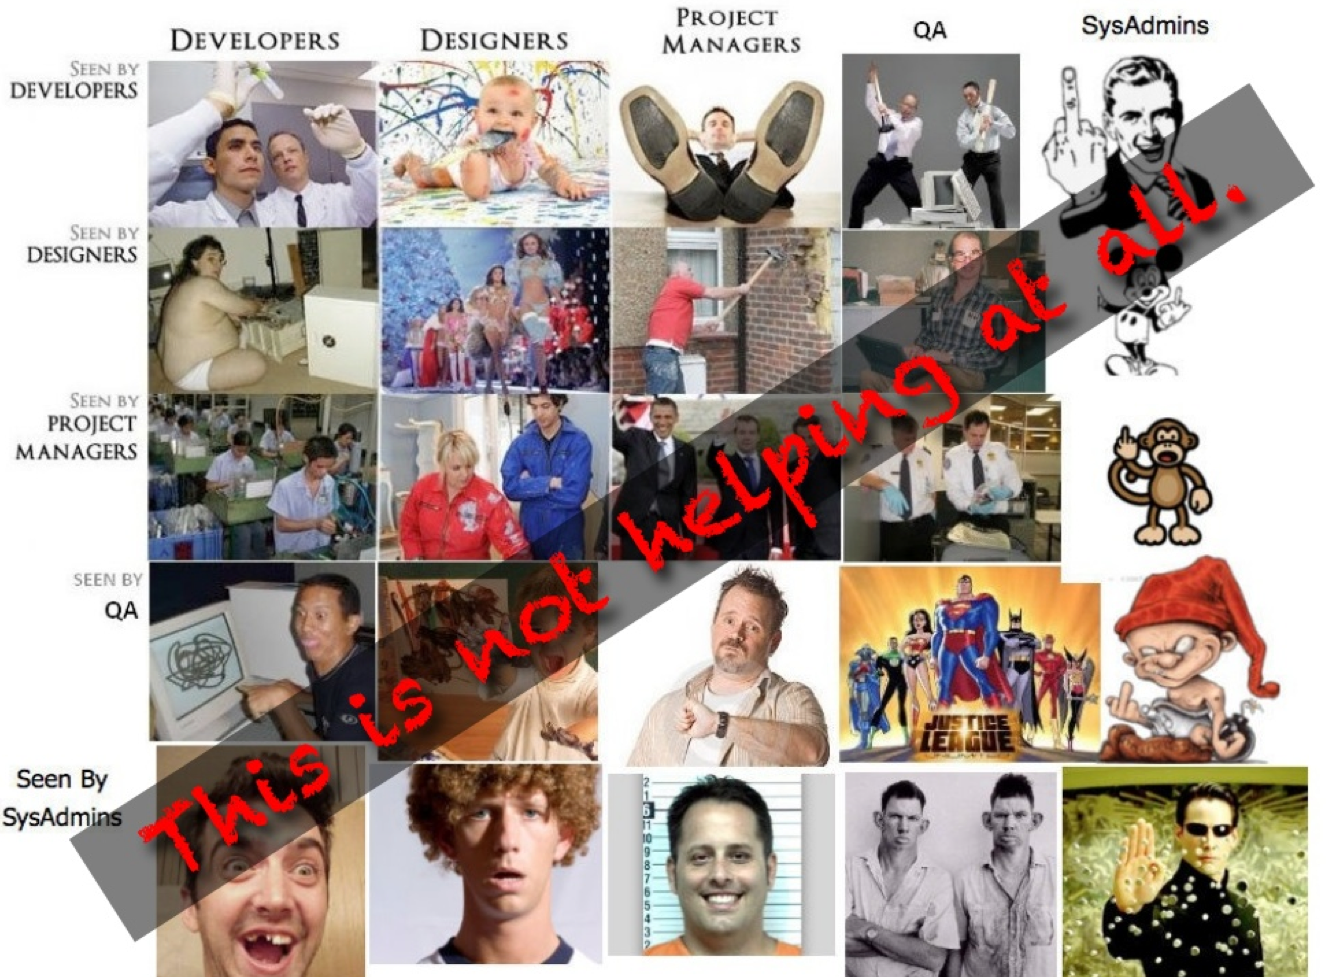
\includegraphics[scale=0.35]{pics/as-seen-by-not-helping.eps} \\
\end{center}
\vspace*{\fill}

\subsection{... and {\em Administration}?}
Merriam Webster:
\begin{quote}
	{\bf administer, v:} {\em to manage or supervise the execution, use, or conduct of} \\
\end{quote}


\subsection{... and {\em Administration}?}
Merriam Webster:
\begin{quote}
	{\bf administer, v:} {\em to manage or supervise the execution, use, or conduct of} \\
\end{quote}

{\em System} Administration frequently also includes other tasks such as
\begin{itemize}
	\item system design and architecture
\end{itemize}

\subsection{... and {\em Administration}?}
Merriam Webster:
\begin{quote}
	{\bf administer, v:} {\em to manage or supervise the execution, use, or conduct of} \\
\end{quote}

{\em System} Administration frequently also includes other tasks such as
\begin{itemize}
	\item system design and architecture
	\item reliability studies
\end{itemize}

\subsection{... and {\em Administration}?}
Merriam Webster:
\begin{quote}
	{\bf administer, v:} {\em to manage or supervise the execution, use, or conduct of} \\
\end{quote}


{\em System} Administration frequently also includes other tasks such as
\begin{itemize}
	\item system design and architecture
	\item reliability studies
	\item resource management
\end{itemize}

\subsection{... and {\em Administration}?}
Merriam Webster:
\begin{quote}
	{\bf administer, v:} {\em to manage or supervise the execution, use, or conduct of} \\
\end{quote}

{\em System} Administration frequently also includes other tasks such as
\begin{itemize}
	\item system design and architecture
	\item reliability studies
	\item resource management
	\item system fault diagnosis
\end{itemize}

\subsection{... and {\em Administration}?} Merriam Webster: \begin{quote} {\bf
administer, v:} {\em to manage or supervise the execution, use, or conduct of}
\\ \end{quote}

{\em System} Administration frequently also includes other tasks such as
\begin{itemize}
	\item system design and architecture
	\item reliability studies
	\item resource management
	\item system fault diagnosis
	\item ...
\end{itemize}


\subsection{... and {\em Administration}?}
Merriam Webster:
\begin{quote}
	{\bf administer, v:} {\em to manage or supervise the execution, use, or conduct of} \\
\end{quote}

{\em System} Administration frequently also includes other tasks such as
\begin{itemize}
	\item system design and architecture
	\item reliability studies
	\item resource management
	\item system fault diagnosis
	\item ...
\end{itemize}
\vspace{.5in}

...all of which my involve a fair amount of {\em software development}, {\em
programming} and {\em scripting}.

\subsection{Learning System Administration}
System Administration is a profession with no fixed career path.

\subsection{Learning System Administration}
System Administration is a profession with no fixed career path.

\begin{itemize}
	\item few degree granting programs
\end{itemize}

\subsection{Learning System Administration}
System Administration is a profession with no fixed career path.

\begin{itemize}
	\item few degree granting programs
	\item heavy reliance on practical experience
\end{itemize}

\subsection{Learning System Administration}
System Administration is a profession with no fixed career path.

\begin{itemize}
	\item few degree granting programs
	\item heavy reliance on practical experience
	\item specializations in many different areas possible
\end{itemize}

\subsection{Learning System Administration}
System Administration is a profession with no fixed career path.

\begin{itemize}
	\item few degree granting programs
	\item heavy reliance on practical experience
	\item specializations in many different areas possible
	\item breadth of expertise as necessary as depth in some areas
\end{itemize}


\subsection{Learning System Administration}
System Administration is a profession with no fixed career path.

\begin{itemize}
	\item few degree granting programs
	\item heavy reliance on practical experience
	\item specializations in many different areas possible
	\item breadth of expertise as necessary as depth in some areas
	\item background knowledge and requirements vary
\end{itemize}

\subsection{Learning System Administration}

Breadth of knowledge:
\begin{itemize}
	\item operating system concepts
	\item TCP/IP networking
	\item programming
	\item ...
\end{itemize}
\vspace{.5in}

Depth of knowledge:
\begin{itemize}
	\item certain OS flavor
	\item specific service (DNS, E-Mail, Databases, Content-Delivery, ...)
	\item specific implementation/vendor (Oracle, Hadoop, Apache, Cisco, ...)
	\item specific are of expertise (security, storage, network, data center, ...)
	\item ...
\end{itemize}

\subsection{People think the internet looks like this.}
\begin{center}
	
\includegraphics[scale=0.7]{pics/cloud.eps}
\end{center}

\subsection{Or like this.}
\begin{center}
	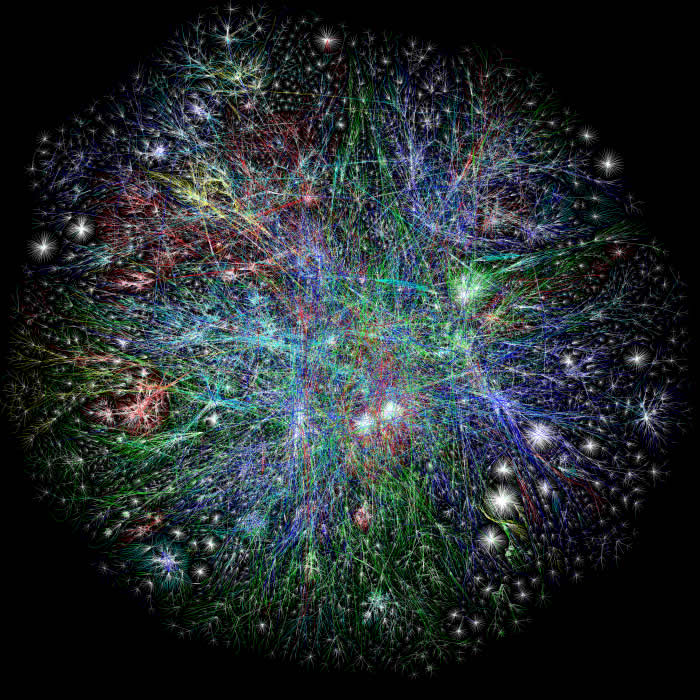
\includegraphics[scale=0.4]{pics/internet.eps} \\
	\small
	{\tt http://www.opte.org/maps/}
	\Normalsize
\end{center}

\subsection{SysAdmins know it looks like this.}
\vspace*{\fill}
\begin{center}
    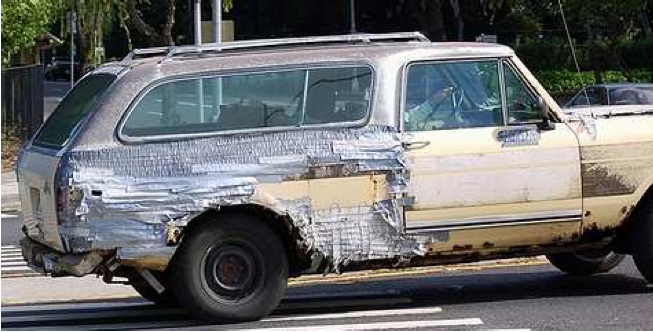
\includegraphics[scale=0.9]{pics/car-duct-tape.eps}
\end{center}
\vspace*{\fill}

\newpage
\vspace*{\fill}
\begin{center}
    \Hugesize
        Hooray! \\ [1em]
    \hspace*{5mm}
    \blueline\\
    \hspace*{5mm}\\
        5 Minute Break
\end{center}
\vspace*{\fill}

\subsection{In reality...}
\vspace*{\fill}
\begin{center}
    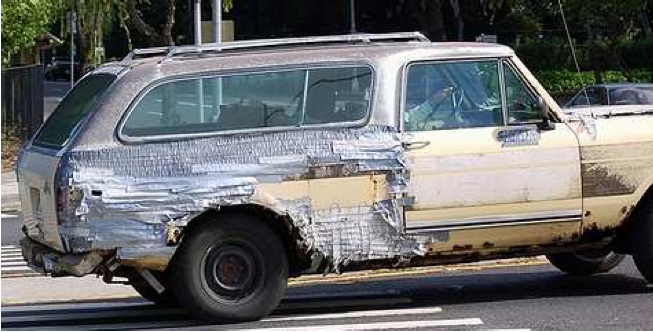
\includegraphics[scale=0.9]{pics/car-duct-tape.eps}
\end{center}
\vspace*{\fill}

\subsection{About this class}
We can only cover {\em some} of the aspects of System Administration.
\vspace*{\fill}
\begin{center}
	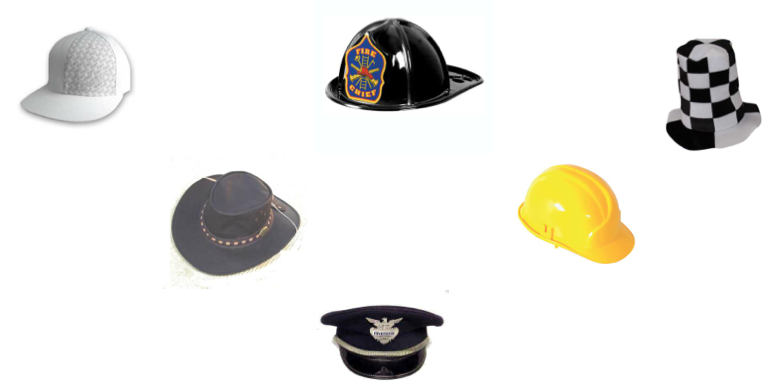
\includegraphics[scale=0.8]{pics/hats.eps}
\Normalsize
\end{center}
\vspace*{\fill}

\subsection{SysAdmins' favorite tool}
\begin{center}
	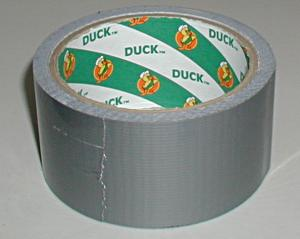
\includegraphics[scale=1.0]{pics/DuckTape.eps} \\
	\vspace{.5in}
	\small
	\verb+https://www.netmeister.org/blog/duct-tape-and-wd40.html+
	\Normalsize
\end{center}

\subsection{Three Pillars of Exceptional System Design}
We will give particular attention to these three core features:
\begin{itemize}
	\item Scalability
	\item Security
	\item Simplicity
\end{itemize}

\subsection{Three Pillars of Exceptional System Design: Scalability}
\vspace*{\fill}
\begin{center}
    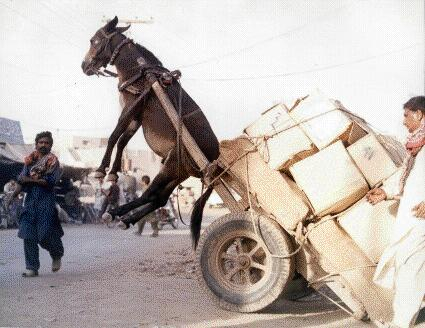
\includegraphics[scale=0.8]{pics/donkey_too_small_for_load.eps} \\
	System Overload
\end{center}
\vspace*{\fill}

\subsection{Three Pillars of Exceptional System Design: Scalability}
\vspace*{\fill}
\begin{center}
    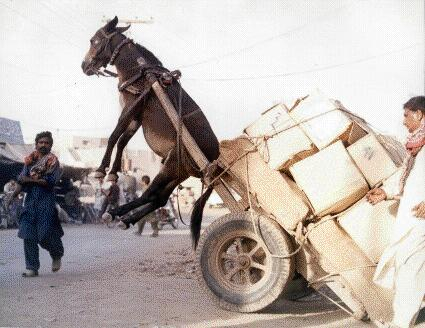
\includegraphics[scale=0.2]{pics/donkey_too_small_for_load.eps} \\
    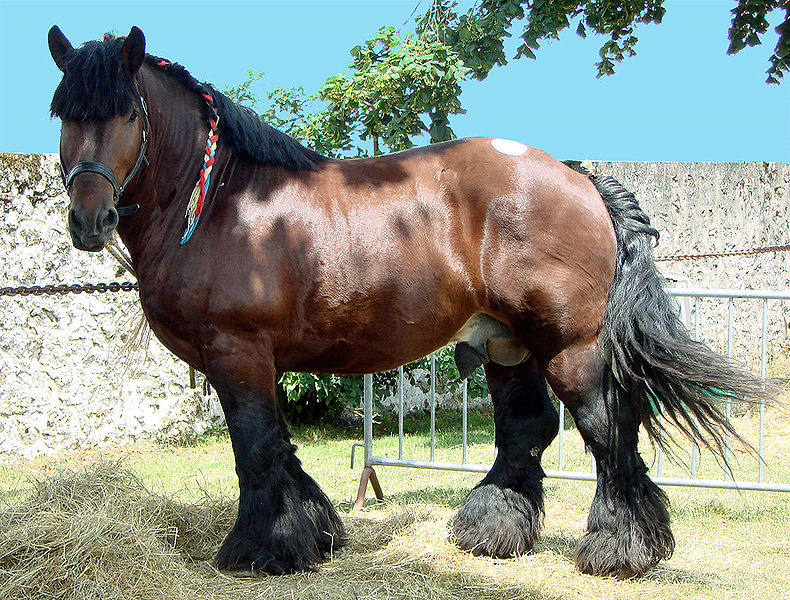
\includegraphics[scale=0.4]{pics/ardennes-horse.eps} \\
	Scaling Vertically
\end{center}
\vspace*{\fill}


\subsection{Three Pillars of Exceptional System Design: Scalability}
\vspace*{\fill}
\begin{center}
    \includegraphics[scale=0.2]{pics/donkey_too_small_for_load.eps} \\
    \includegraphics[scale=0.5]{pics/vierspaenner.eps} \\
	Scaling Horizontally
\end{center}
\vspace*{\fill}

\subsection{Three Pillars of Exceptional System Design: Scalability}
\vspace*{\fill}
\begin{center}
    \includegraphics[scale=0.2]{pics/donkey_too_small_for_load.eps} \\
    \includegraphics[scale=1.1]{pics/dogcart.eps} \\
	Scaling Down
\end{center}
\vspace*{\fill}

\subsection{Three Pillars of Exceptional System Design: Security}
\vspace*{\fill}
\begin{center}
    \includegraphics[scale=1.4]{pics/usability-security.eps} \\
\end{center}
\vspace*{\fill}

\subsection{Three Pillars of Exceptional System Design: Security}
\vspace*{\fill}
\begin{center}
    \includegraphics[scale=1.0]{pics/patch-bandaid.eps} \\
\end{center}
\vspace*{\fill}

\subsection{Three Pillars of Exceptional System Design: Security}
\vspace*{\fill}
\begin{center}
    \includegraphics[scale=1.4]{pics/wrong-usability.eps} \\
\end{center}
\vspace*{\fill}

\subsection{Three Pillars of Exceptional System Design: Security}
\vspace*{\fill}
\begin{center}
    \includegraphics[scale=1.1]{pics/better-usability.eps} \\
	\small
	{\tt https://www.netmeister.org/blog/infosec-basics.html}
	\Normalsize
\end{center}
\vspace*{\fill}


\subsection{Three Pillars of Exceptional System Design: Simplicity}
\vspace*{\fill}
\begin{center}
    \includegraphics[scale=0.3]{pics/kiss.eps} \\
\end{center}
\vspace*{\fill}

\subsection{Three Pillars of Exceptional System Design: Simplicity}
\vspace*{\fill}
\begin{center}
    \includegraphics[scale=1.2]{pics/lego-block.eps} \\
\end{center}
\vspace*{\fill}

\subsection{Three Pillars of Exceptional System Design: Simplicity}
\vspace*{\fill}
\begin{center}
    \includegraphics[scale=0.1]{pics/millennium-falcon.eps} \\
\end{center}
\vspace*{\fill}

\subsection{SysAdmins' favorite Laws}
\smallish
Ockham's Razor:
\begin{quote}
{\em ``Of two equivalent theories or explanations, all other things being
equal, the simpler one is to be preferred.''}
\end{quote}
\Normalsize

\subsection{SysAdmins' favorite Laws}
\smallish
Ockham's Razor:
\begin{quote}
{\em ``Of two equivalent theories or explanations, all other things being
equal, the simpler one is to be preferred.''}
\end{quote}

2nd Law of Thermodynamics:
\begin{quote}
{\em ``The entropy of an isolated system always increases with time.''}
\end{quote}
\Normalsize

\subsection{SysAdmins' favorite Laws}
\smallish
Ockham's Razor:
\begin{quote}
{\em ``Of two equivalent theories or explanations, all other things being
equal, the simpler one is to be preferred.''}
\end{quote}

2nd Law of Thermodynamics:
\begin{quote}
{\em ``The entropy of an isolated system always increases with time.''}
\end{quote}

Hanlon's Razor:
\begin{quote}
{\em ``Never attribute to malice that which can be adequately explained by
stupidity.''}
\end{quote}
\Normalsize

\subsection{SysAdmins' favorite Laws}
\smallish
Ockham's Razor:
\begin{quote}
{\em ``Of two equivalent theories or explanations, all other things being
equal, the simpler one is to be preferred.''}
\end{quote}

2nd Law of Thermodynamics:
\begin{quote}
{\em ``The entropy of an isolated system always increases with time.''}
\end{quote}

Hanlon's Razor:
\begin{quote}
{\em ``Never attribute to malice that which can be adequately explained by
stupidity.''}
\end{quote}

Pareto's Principle:
\begin{quote}
{\em ``80\% of consequences stem from 20\% of the causes.''}
\end{quote}
\Normalsize

\subsection{SysAdmins' favorite Laws}
\smallish
Ockham's Razor:
\begin{quote}
{\em ``Of two equivalent theories or explanations, all other things being
equal, the simpler one is to be preferred.''}
\end{quote}

2nd Law of Thermodynamics:
\begin{quote}
{\em ``The entropy of an isolated system always increases with time.''}
\end{quote}

Hanlon's Razor:
\begin{quote}
{\em ``Never attribute to malice that which can be adequately explained by
stupidity.''}
\end{quote}

Pareto's Principle:
\begin{quote}
{\em ``80\% of consequences stem from 20\% of the causes.''}
\end{quote}

Sturgeon's Law:
\begin{quote}
{\em ``90\% of everything is crud.''}
\end{quote}
\Normalsize

\subsection{SysAdmins' favorite Laws}
\smallish
Ockham's Razor:
\begin{quote}
{\em ``Of two equivalent theories or explanations, all other things being
equal, the simpler one is to be preferred.''}
\end{quote}

2nd Law of Thermodynamics:
\begin{quote}
{\em ``The entropy of an isolated system always increases with time.''}
\end{quote}

Hanlon's Razor:
\begin{quote}
{\em ``Never attribute to malice that which can be adequately explained by
stupidity.''}
\end{quote}

Pareto's Principle:
\begin{quote}
{\em ``80\% of consequences stem from 20\% of the causes.''}
\end{quote}

Sturgeon's Law:
\begin{quote}
{\em ``90\% of everything is crud.''}
\end{quote}

Murphy's Law:
\begin{quote}
{\em ``If it can happen, it will happen.''}
\end{quote}
\Normalsize


\subsection{SysAdmins' favorite Laws}
\smallish
Ockham's Razor:
\begin{quote}
{\em ``Of two equivalent theories or explanations, all other things being
equal, the simpler one is to be preferred.''}
\end{quote}

2nd Law of Thermodynamics:
\begin{quote}
{\em ``The entropy of an isolated system always increases with time.''}
\end{quote}

Hanlon's Razor:
\begin{quote}
{\em ``Never attribute to malice that which can be adequately explained by
stupidity.''}
\end{quote}

Pareto's Principle:
\begin{quote}
{\em ``80\% of consequences stem from 20\% of the causes.''}
\end{quote}

Sturgeon's Law:
\begin{quote}
{\em ``90\% of everything is crud.''}
\end{quote}

Murphy's Law:
\begin{quote}
{\em ``If it can happen, it will happen.''}
\end{quote}

Throw in some philosophy for good measure:
\begin{quote}
{\em Causality: For every effect, there must be a cause.}
\end{quote}
\Normalsize

\subsection{Learning is critical}
Know how to find answers:
\begin{itemize}
	\item know {\em how} to ask questions
	\item know {\em where} to ask questions
	\item read critically
	\item know what you don't know (Dunning-Kruger effect)
	\item understand {\em what} you're doing
	\item understand {\em why} you're doing it
	\item seek information exchange
\end{itemize}

\subsection{Learning is critical}
\vspace{1in}
\Huge
\begin{center}
``Computer Science projects are opportunities,
not assignments.'' \\
\vspace{.5in}
\verb+http://codeorg.tumblr.com/post/110291421258/sotw26+
\end{center}
\Normalsize

\subsection{Learning is critical}
Know how to find answers:
\begin{itemize}
	\item know {\em how} to ask questions
	\item know {\em where} to ask questions
	\item read critically
	\item know what you don't know (Dunning-Kruger effect)
	\item understand {\em what} you're doing
	\item understand {\em why} you're doing it
	\item seek information exchange
\end{itemize}
\vspace{.5in}
\verb+https://www.cs.stevens.edu/~jschauma/615/s15-meetup.html+

\subsection{Let's review HW1}
{\tt http://www.cs.stevens.edu/\~{}jschauma/615/s15-hw1.html} \\
\vspace{.5in}

Running an instance:
\begin{verbatim}
$ aws ec2 run-instances --key-name stevens --security-groups stevens \
        --image-id <AMI-ID>
\end{verbatim}

\subsection{Let's review HW1}
{\tt http://www.cs.stevens.edu/\~{}jschauma/615/s15-hw1.html} \\
\vspace{.5in}

Save yourself some typing:
\begin{verbatim}
$ alias instance='aws ec2 run-instances --key-name stevens \
                        --security-groups stevens --image-id'
$ instance <AMI-ID>
\end{verbatim}

\subsection{Let's review HW1}
{\tt http://www.cs.stevens.edu/\~{}jschauma/615/s15-hw1.html} \\
\vspace{.5in}


Make it permanent:
\begin{verbatim}
$ echo "alias instance='aws ec2 run-instances --key-name stevens \
        --security-groups stevens --image-id'" >> .bashrc
\end{verbatim}


\subsection{Let's review HW1}
{\tt http://www.cs.stevens.edu/\~{}jschauma/615/s15-hw1.html} \\
\vspace{.5in}

ssh to an instance:
\begin{verbatim}
$ ssh -i ~/.ec2/stevens.pem root@<mumble>.compute-1.amazonaws.com
\end{verbatim}


\subsection{Let's review HW1}
{\tt http://www.cs.stevens.edu/\~{}jschauma/615/s15-hw1.html} \\
\vspace{.5in}

Let's save ourselves some typing:
\begin{verbatim}
$ cat >>~/.ssh/config <<EOF
> Host *.amazonaws.com
>         IdentityFile ~/.ec2/stevens.pem
>         User         root
> EOF
$ ssh <mumble>.compute-1.amazonaws.com
\end{verbatim}


\subsection{Filesystems, Disk, Storage}
\begin{verbatim}
$ instance ami-35eb835c
[...]
$ aws ec2 describe-instances
[...]
$ ssh root@ec2-54-198-235-45.compute-1.amazonaws.com
\end{verbatim}

\subsection{Let's review HW1}
\begin{verbatim}
# uname -a
SunOS domU-12-31-39-0F-1C-BB.compute-1.internal 5.11 omnios-33fdde4 i86pc
i386 i86xpv Solaris
#
\end{verbatim}

\subsection{Let's review HW1}
\begin{verbatim}
# ifconfig -a
lo0: flags=2001000849<UP,LOOPBACK,RUNNING,MULTICAST,IPv4,VIRTUAL> mtu 8232 index 1
        inet 127.0.0.1 netmask ff000000
xnf0: flags=1004843<UP,BROADCAST,RUNNING,MULTICAST,DHCP,IPv4> mtu 1500 index 2
        inet 10.110.94.225 netmask fffffe00 broadcast 10.110.95.255
        ether 12:31:39:1c:60:13
lo0: flags=2002000849<UP,LOOPBACK,RUNNING,MULTICAST,IPv6,VIRTUAL> mtu 8252 index 1
        inet6 ::1/128
xnf0: flags=20002000840<RUNNING,MULTICAST,IPv6> mtu 1500 index 2
        inet6 ::/0
        ether 12:31:39:1c:60:13
#
\end{verbatim}


\subsection{Let's review HW1}
\begin{verbatim}
# netstat -na | more
[...]
TCP: IPv4
   Local Address        Remote Address    Swind Send-Q Rwind Recv-Q
State
-------------------- -------------------- ----- ------ ----- ------ -----------
127.0.0.1.4999             *.*                0      0 128000      0 LISTEN
      *.111                *.*                0      0 128000      0 LISTEN
      *.*                  *.*                0      0 128000      0 IDLE
      *.111                *.*                0      0 128000      0 LISTEN
      *.*                  *.*                0      0 128000      0 IDLE
      *.46457              *.*                0      0 128000      0 LISTEN
      *.55986              *.*                0      0 128000      0 LISTEN
      *.22                 *.*                0      0 128000      0 LISTEN
10.110.94.225.22     155.246.89.107.46137 42304     47 128592      0 ESTABLISHED
[...]
\end{verbatim}

\subsection{Let's review HW1}
\begin{verbatim}
# man df
[...]
# df
[...]
# df -hT
[...]
# df -i
[...]
# df -a
[...]
# mount
[...]
\end{verbatim}


\subsection{Let's review HW1}
\begin{verbatim}
# format
[...]
format> verify
[...]
# zpool list
[...]
# zfs list
[...]
\end{verbatim}

\newpage
\vspace*{\fill}
\begin{center}
    \Hugesize
        The End \\ [1em]
    \hspace*{5mm}
    \blueline\\
    \hspace*{5mm}\\
        Hooray!
\end{center}
\vspace*{\fill}

\subsection{Reading}
Miscellaneous:
\begin{itemize}
	\item \verb+http://www.opsschool.org/+
	\item \verb+http://nixsrv.com/llthw+
	\item \verb+http://linuxcommand.org/lc3_learning_the_shell.php+
	\item \verb+http://www.sage.org/pubs/22_jobs/+
\end{itemize}

UNIX history:
\begin{itemize}
	\item \verb+http://www.bell-labs.com/history/unix/+
	\item \verb+http://www.futuretech.blinkenlights.nl/admin/day1a.html+
	\item \verb+http://www.levenez.com/unix/+
	\item \verb+https://en.wikipedia.org/wiki/Operating_system+
\end{itemize}

\subsection{Reading}
UNIX basics:
\begin{itemize}
	\item chmod(1), chown(1), ls(1)
	\item intro(1), login(1), passwd(5)
	\item su(1), sudo(8)
\end{itemize}

%\nocite{*}
%\bibliographystyle{plain}
%\bibliography{slides}

\end{document}
